\section{Focchi, Semini et al. - Robot Impedance Control and Passivity Analysis
with Inner Torque and Velocity Feedback Loops \cite{SeminiFocchi2}}
Authors: Michele Focchi\\
Year: 2014
\subsection*{Summary}
The interest of this paper is to identify the values of the parameters which yield a stable impedance in the system. In particular the focus is given to the HAA joint of HyQ.\\
The controller is a nested structure of three layers:
\begin{itemize}
\item inner positive feedback control loop (velocity compensation gain $\alpha$). Here the velocity is obtained through derivative of the angular join position which yields highly noisy signals, as a consequence also a filter needs to be introduced, parametrized by $N_{av}$, to smooth the signal.
\item torque loop (proportional feedback gain $\beta$)
\item outer impedance control (PD controller with $P_{gain}$ and $D_{gain}$)
\end{itemize}
Besides the 5 parameters mentioned above also the sampling time $t_s$ has got a high influence on the stability of the system.\\
The stability analysis is here carried out highlighting the \textbf{passivity} property of the system. Passivity is a conservative condition which states that given a passive system (such as an obstacle in the environment) the robot interaction with that system will be stable if it also behaves in a passive way. Passive springs are always passive in that they induce energy dissipation, but an active compliant system may be passive only under a proper analysis. In this paper it is shown that a \textbf{driving port impedance transfer function} $Z(s)$ will be positive only under the two following conditions:
\begin{enumerate}
\item $Z(s)$ has no pole with positive real part
\item the phase of $Z(s)$ lies between -90 and 90$\degree$
\end{enumerate}
\begin{figure}
  \centering
  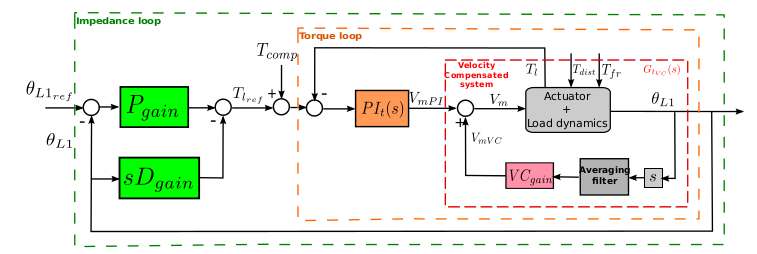
\includegraphics[width=120mm]{VelocityAndTorqueControl}
  \caption{Block diagram of the velocity compensated system with inner torque loop and outer impedance loop}
  \label{SpeedTorqueControl}
\end{figure}
In the paper is also explained that, due to the derivative operator, the velocity compensator does not only influence the poles of the c.l.system (as the torque loop does), but it also affects the zeros of the system.
\subsection*{Key points / Takeaways}
\begin{itemize}
\item compliance might be limited by the bandwidth of inner control loops (such as torque control loops by instance). The \textbf{bandwidth} is defined as the frequency where the torque amplitude decreases by $-3$dB with respect to the reference system.
\item When we have a cascade of control loops it becomes fundamental to test the correct bandwidth of each loop. The bandwidth of the loop is connected to the time response, or more precisely, to the rise time in this way: $$ f(Hz) = \frac{1}{t_r(sec)}$$
In general in cascaded control loops we have that the \textbf{bandwidth} of the innermost loop as to be at least one order of magnitude faster than the outer loop. The higher the bandwidth (faster system) the better the tracking error, whilst the lower the bandwidth (for slow systems) the higher the \textbf{damping effect}. In robotic systems where we are interested in achieving compliant behaviors, the bandwidth must be tuned in order to find a trade-off between \textbf{tracking} error and impedance.\\
The bandwidth is directly affected by \textbf{sampling frequency} $T_s$ and \textbf{filtering} $N_{av}$ (number of samples to be filtered together): the lower the frequency of the system, the slower the system, the lower the bandwidth.\\
Usually in \textbf{nested control loops} the slowest frequency acts as a \textbf{bottleneck} for the whole system.
\item It is better to discretize the system and carry out the analysis in discrete domain because discretizing introduces many problems; for example a minimum phase system may become \textbf{non-minimum phase} when it is discretized.
\item Sampling time of the controller: $t_s=$ 1 ms
\item The compliance controller can be seen as nothing but the tracking of the joint angle with more or less high PD gains. High $P_{gain}$ and $D_{gain}$ will result in stiff behavior (low compliance) while low gains will result in high compliance.
\end{itemize}
\subsection*{Weak points}
\subsection*{Ideas}